\documentclass[fleqn,10pt]{wlscirep}

\usepackage{chemformula}
\usepackage{amsmath}
\usepackage[]{mcode}

\title{Stochastic Dynamics of RNA interference: A Single-Molecule Time-based Approach}

\author[1*]{Baihan Lin}
\author[1]{Hong Qian}
\affil[1]{Department of Applied Mathematics, University of Washington, Seattle, WA 98195, USA}
\affil[*]{doerlbh@gmail.com}

\keywords{RNA interference, Central dogma, Stochastic gene expression, Chemical master equation, Single molecule}

\begin{abstract}

Under a general mechanistic understanding of RNA interference, we present a stochastic model for the cellular dynamics of gene expression involved in RNA interference in a single-molecule time-based approach. Although the mechanistic model is constructed under various simplifications and assumptions to decrease the innate diversity and complexity in RNA interference behaviors, considering the introduction of single-molecule approach introduced into this system, the biological implication is still a worthwhile effort. Both the deterministic model and stochastic model demonstrate similar equilibrium. A Monte Carlos simulation method is also introduced to support chemical master equation. Although this is not the first paper to establish a stochastic theory in RNA level, the understanding of stochastic behavior and how it compares with the traditional deterministic approach still offers certain insights into a non-closed biochemical system. 

\end{abstract}
\begin{document}

\flushbottom
\maketitle
%\thispagestyle{empty}

\section*{Introduction}

RNA interference (RNAi) is an important biological process in which RNA molecules inhibit gene expression. Although in different mechanisms, typically these noncoding RNA molecules causes the destruction of specific messenger RNA (mRNA) molecules. \cite{MacRae195}. As shown in Figure \ref{fig:diagram}, the RNA interference can be simplified as a genetic circuit, where central dogma determines that one set of DNA was transcribed into messenger RNA (mRNA) and interfering RNA (iRNA), mRNA were translated to protein, while iRNA inhibit the translation of mRNA.

Inspired by the single-molecule approach applied to probe the stochastic gene expression with respect to transcription factor \cite{Elf1191} and stochastic gene state switching \cite{PhysRevLett.114.078101}, we proposed a single-molecule theory of stochastic gene expression on RNA-based regulation, starting from interference system of siRNA and microRNA which reversibly inhibits mRNA transcription with increased degradation. 

microRNA (miRNA) and small interfering RNA (siRNA) two types of small RNA molecules central to RNA interference. Take microRNA as an example: a protein called exportin-5 transports a hairpin primary microRNA (pri-miRNA) out of nucleus; an enzyme called dicer trimes pri-miRNA and removes hairpin loop, exposing one strand to join a group of proteins forming microRNA-protein complex; the microRNA-protein complex binds with mRNA strand, to produce a RNA-induced silencing complex (RISC), which stops translation process; the prescence of microRNA-protein complex blocks translation as well as speeding up deadenylation, which is a process to breakdown Poly-A tail and cause mRNA to be degraded sooner and translated less. siRNA's regulatory pathway is similar to microRNA.

\begin{figure}[ht]
\centering
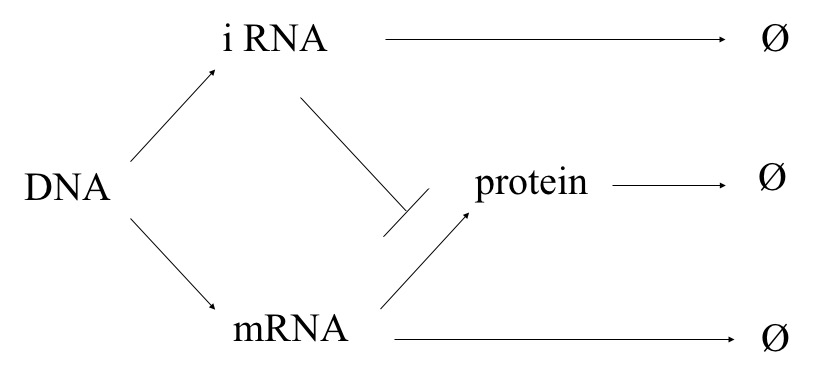
\includegraphics[width=6cm]{diagram}
\caption{a diagram for the genetic circuit simplification of RNA interference}
\label{fig:diagram}
\end{figure}


\section*{Results}

To simply the model, we used iRNA to represent microRNA and siRNA, which are similar RNA interference agents. Instead of producing transcription factor to bind with DNA, iRNA tends to bind with mRNA and form a complex to inhibit the translation. 

The chemical reactions involved in this process is therefore summarized as these 8 steps:

\begin{itemize}
\item \ch{DNA + NTPs ->[k1] DNA + mRNA}
\item \ch{DNA + NTPs ->[k2] DNA + iRNA}
\item \ch{mRNA + AAs ->[k3] mRNA + protein}
\item \ch{mRNA + iRNA + RISC <=>[h][f] mRNA.iRNA.RISC}
\item \ch{mRNA ->[$\gamma$1] $\emptyset$}
\item \ch{iRNA ->[$\gamma$1] $\emptyset$}
\item \ch{mRNA.iRNA.RISC ->[$\gamma$2] $\emptyset$}
\item \ch{protein ->[$\gamma$3] $\emptyset$}
\end{itemize}
 
where NTPs stand for nucleoside triphosphates, which are building blocks for RNA, and AAs stand for amino acid, which are building blocks for protein.
 
\subsection*{Deterministic Dynamics and Non-equilibrium Steady States}

To simplify our model, we made several assumptions: 
\begin{itemize}
\item we assume same degradation rate for iRNA and mRNA;
\item we assume an irreversible inhibition, which means h $\gg$ f;
\item we assume the degradation rate of bound mRNA higher than mRNA and iRNA;
\item we assume the concentrations of DNA, AAs, NTPs, RISCs are abundant and can be considered to be maintained.
\item we assume no other regulation behavior (such as transcription factors etc.)
\end{itemize}

Based on above reactions, following the law of mass action, the ordinary differential equation can be written:

\begin{equation}
\frac{d[iRNA]}{dt} = k_2[DNA][NTPs] - \gamma_1[iRNA] + f[mRNA.iRNA.RISC] - h[RISCs][iRNA][mRNA] 
\end{equation}
\begin{equation}
\frac{d[mRNA]}{dt} = k_1[DNA][NTPs] - \gamma_1[mRNA] + f[mRNA.iRNA.RISC] - h[RISCs][iRNA][mRNA]  
\end{equation}
\begin{equation}
\frac{d[mRNA.iRNA.RISC]}{dt} = - \gamma_2[mRNA.iRNA.RISC] + h[RISCs][iRNA][mRNA] 
\end{equation}
\begin{equation}
\frac{d[protein]}{dt} = k_3[mRNA][NTPs] - \gamma_3[protein]
\end{equation}

Since the concentrations of DNA, AAs, NTPs, RISCs can be considered to be maintained in the cell, we can simplify the system by denoting:

\begin{equation}
K_1 = k_1[mRNA][NTPs], K_2 = k_2[mRNA][NTPs], K_3 = k_3[AAs], H = h[RISCs]
\end{equation}

If we denote the concentrations of iRNA , mRNA, mRNA.iRNA.RISC and protein at time t, denoted as x(t), y(t), z(t), w(t), then the differential equations can be rewritten as:
\begin{equation}
\frac{dx}{dt} = K_2 - \gamma_1x + fz - Hxy 
\end{equation}
\begin{equation}
\frac{dy}{dt} = K_1 - \gamma_1y + fz - Hxy
\end{equation}
\begin{equation}
\frac{dz}{dt} = - \gamma_2z + Hxy 
\end{equation}
\begin{equation}
\frac{dw}{dt} = K_3y - \gamma_3w
\end{equation}

If we nondimensionalize all the variables by setting
\begin{equation}
v = \frac{\gamma_1}{K_2}x,   
r = \frac{\gamma_1}{K_1}y,  
q = \gamma_2Hz,  
s = \frac{\gamma_1\gamma_3}{K_1K_3}w,  
\tau = \gamma_3t.
\end{equation}

We get:
\begin{equation}
\frac{dv}{d\tau} = \epsilon_1 (1 - v - H_1vr) = f(v, r)
\end{equation}
\begin{equation}
\frac{dr}{d\tau} = \epsilon_1 (1 - r - H_2vr) = g(v, r)
\end{equation}
\begin{equation}
\frac{dq}{d\tau} = \epsilon_2 (- q + H_3vr)
\end{equation}
\begin{equation}
\frac{ds}{d\tau} = r - s
\end{equation}

where 
\begin{equation}
\epsilon_1 = \frac{\gamma_2}{\gamma_3}, 
\epsilon_2 = \frac{\gamma_1}{\gamma_3}, 
H_1 = H\frac{K_1}{\gamma_1\gamma_3}, 
H_2 = H\frac{K_2}{\gamma_1\gamma_3}, 
H_3 = \epsilon_1H^2\frac{K_1K_2}{\gamma_1^2}.
\end{equation}

To obtain steady states, we set $f(v*, r*) = g(v*, r*) = 0$:
\begin{equation}
v* = \frac{1}{1 + H_1r*}
\end{equation}
\begin{equation}
r* = \frac{1}{1 + H_2v*} = \frac{1}{1 + H_2v*} = \frac{1}{1 + H_2\frac{1}{1 + H_1r*}} = \frac{1 + H_1r*}{1 + H_2v* + H_2} 
\end{equation}

Solving this quadratic equation, we get the analytical steady states as:
\begin{equation}
v* = \frac{H_2 - H_1 - 1 + \sqrt{(H_2 - H_1 - 1)^2 + 4H_2}}{2H_2}
\end{equation}
\begin{equation}
r* = \frac{H_1 - H_2 - 1 + \sqrt{(H_1 - H_2 - 1)^2 + 4H_1}}{2H_1}
\end{equation}
in which there is only one real positive steady state, and the protein production correspondent have a steady state of \begin{equation}
s* = r* + (s(0) - r)*e^{-\tau}
\end{equation}
There is no bifurcation behavior in this deterministic system.

%As shown in Figure \ref{fig:deterss}, 

\begin{figure}[ht]
\centering
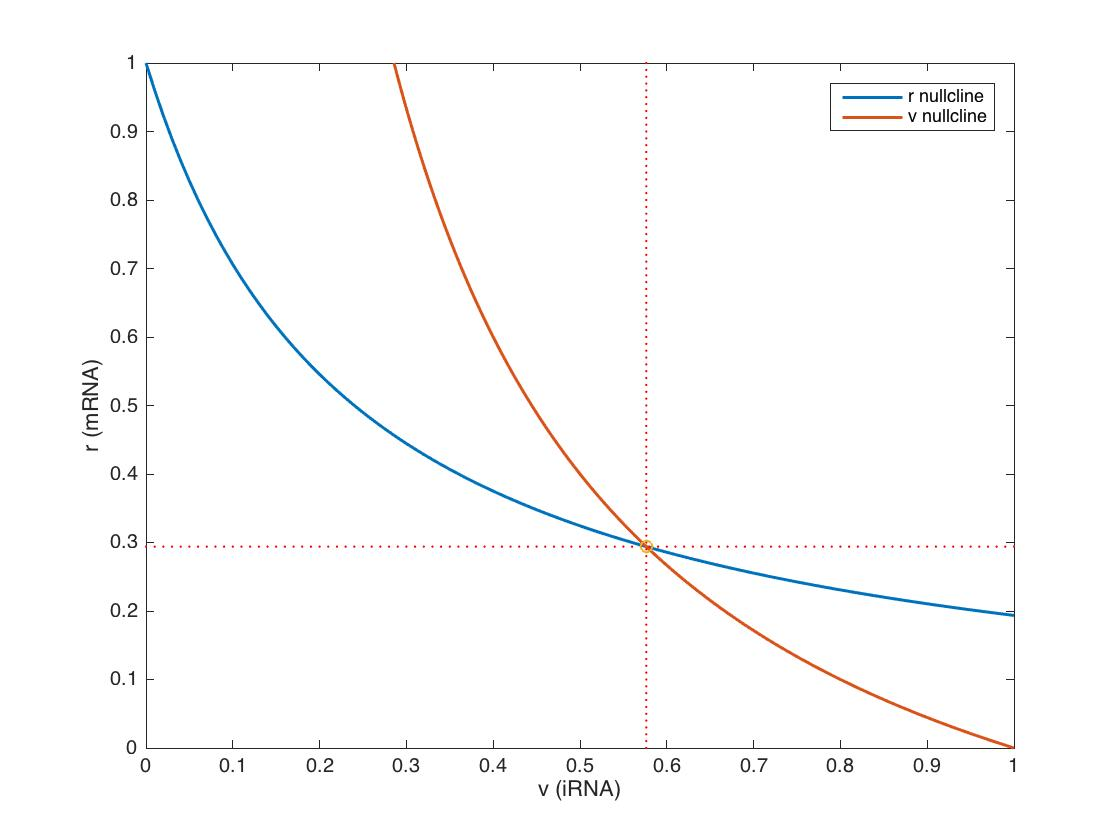
\includegraphics[width=9cm]{deterss}
\caption{the phase portrait of the nondimensionalized system derives one real positive steady state calculated based on the nullclines.}
\label{fig:deterss}
\end{figure}

%As shown in Figure \ref{fig:deterdyn}

\begin{figure}[ht]
\centering
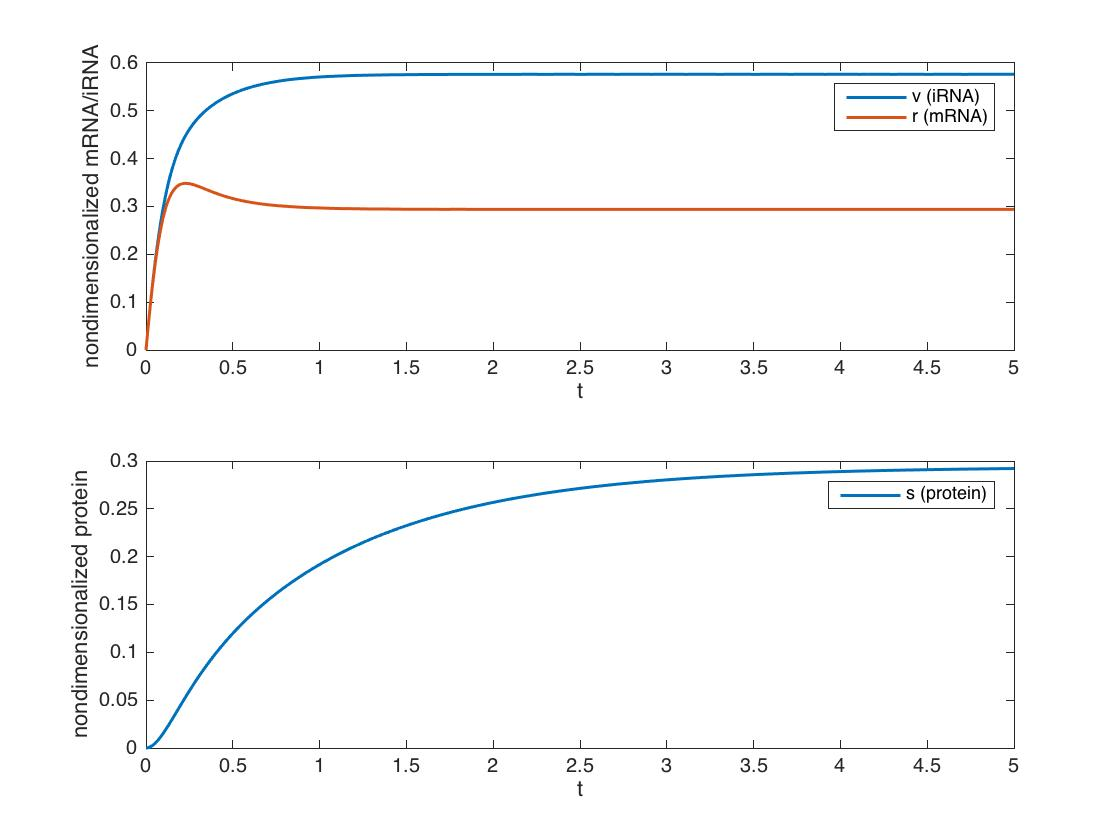
\includegraphics[width=9cm]{deterdyn}
\caption{the deterministic dynamics of the system of mRNA, iRNA and protein.}
\label{fig:deterdyn}
\end{figure}

\subsection*{Chemical Master Equation and Single-Molecule Kinetics}


The chemical master equation of this system can be specified as:
\begin{equation}
\begin{aligned}
\frac{dP(m,n,p)}{dt} = K_2P(m, n - 1, p) + K_1P(m - 1, n, p) + mK_3P(m, n, p - 1) \\ + [(n + 1)\gamma_1 + m(n + 1)H]P(m, n + 1, p)  \\ + (p + 1)\gamma_3P(m, n, p + 1) + [(m + 1)\gamma_1 + (m + 1)nH]P(m + 1, n, p)\\ - P(m, n, p)(K_2 + P\gamma_3 + K_1 + mK_3 + n\gamma_1 + mnH + m\gamma_1 + mnH)
\end{aligned}
\end{equation}
\begin{equation}
\begin{aligned}
\frac{dP(0,n,p)}{dt} = K_2P(0, n - 1, p) +  (n + 1)\gamma_1P(0, n + 1, p) + (p + 1)\gamma_3P(0, n, p + 1) \\+ (\gamma_1 + nH)P(1, n, p) - P(0, n, p)(K_2 + P\gamma_3 + K_1 + n\gamma_1)
\end{aligned}
\end{equation}
\begin{equation}
\begin{aligned}
\frac{dP(m,0,p)}{dt} = K_1P(m - 1, 0, p) + mK_3P(m, 0, p - 1) + [\gamma_1 + mH]P(m, 1, p) \\+ (p + 1)\gamma_3P(m, 0, p + 1) + (m + 1)\gamma_1P(m + 1, 0, p) \\- P(m, 0, p)(K_2 + P\gamma_3 + K_1 + mK_3 + m\gamma_1)
\end{aligned}
\end{equation}
\begin{equation}
\begin{aligned}
\frac{dP(m,n,0)}{dt} = K_2P(m, n - 1, -) + K_1P(m - 1, n, 0)+ [(n + 1)\gamma_1 + m(n + 1)H]P(m, n + 1, 0)\\ + \gamma_3P(m, n, 1) + [(m + 1)\gamma_1 + (m + 1)nH]P(m + 1, n, 0) \\- P(m, n, 0)(K_2 + P\gamma_3 + K_1 + mK_3 \\+ n\gamma_1 + mnH + m\gamma_1 + mnH)
\end{aligned}
\end{equation}

As shown in Figure \ref{fig:cme}, the transition diagram is in 3 dimensions, in the number of iRNA molecule, mRNA molecule, and protein molecule. Different from the stochastic system of transcription factor, the iRNA and mRNA axes are independent of protein axis.

\begin{figure}[ht]
\centering
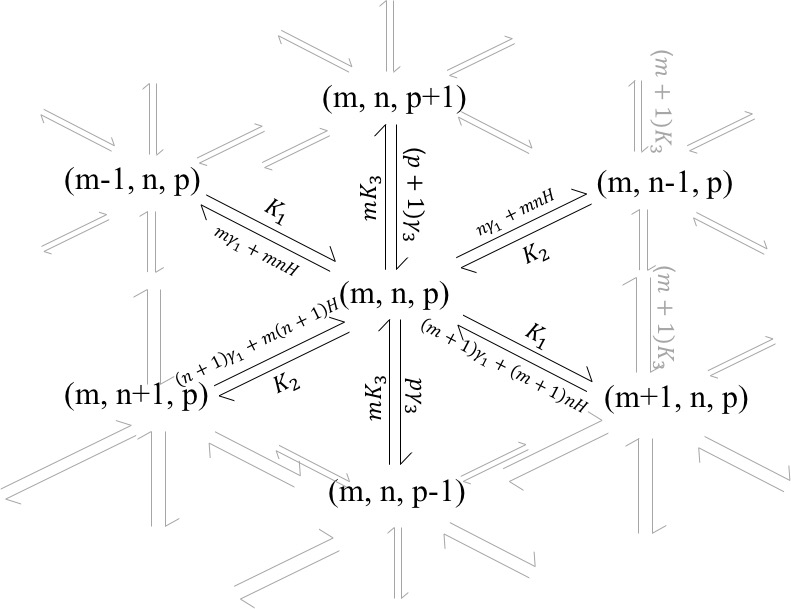
\includegraphics[width=\linewidth]{cme}
\caption{a discrete schematic illustrating the Markovian kinetics of a single molecule of iRNA, mRNA, or protein with conformational fluctuations.}
\label{fig:cme}
\end{figure}

However, without accessible experimental data from single-molecule measurement of RNA interference to provide insights into the probability distribution of the system with respect to mRNA, iRNA and protein, we cannot produce probabilities generating functions to analytically solve the entire system.

Therefore, we took a different approach towards this system. If we consider all the reactions involved in this system (synthesis, transcription, regulation, translation and degradation) as independent reactions, then under the single-molecule level, within a high resolution of measurement, only one reaction can happen at the same time. Thus, we can assume a Poisson distribution of the waiting time until next reaction

For each reaction type, the mean time till the next reaction occurs again is the inverse of the reaction rate.  Since the rate at which anything will happen is simply the sum of all the reaction rates, which we'll denote by $\lambda$ as shown as Figure \ref{fig:rate}, we also can write the mean time until any reaction occurs as   
    
\begin{figure}[ht]
\centering
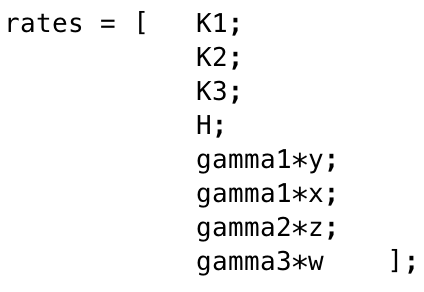
\includegraphics[width=4cm]{rate}
\caption{the reaction rates for each reaction.}
\label{fig:rate} 
\end{figure}
   
    \begin{align*}
        \tau_m = \frac{1}{\lambda}    
    \end{align*}
    
Then, under the assumption of a Poisson process, it's fairly straightforward to pick the next most likely reaction and the amount of time until the reaction occurs. For the time, we have
    
    \begin{align*}
        \tau = \frac{1}{\lambda}\log(\frac{1}{U_1})
    \end{align*}
    
for $U_1$ drawn uniformly from the unit interval.  Likewise, if we denote the individual reaction rates as $a_i$ we can select one based on the relative reaction rates by choosing a random variable
    
    \begin{align*}
        r = \lambda*U_2
    \end{align*}
    
which gives for $U_2$ drawn uniformly from the unit interval. This gives us a random variable in the range $(0, \lambda)$  which we can use to select the next reaction $j$ by finding $j$ such that
    
    \begin{align*}
        \sum\limits_0^{j-1} \leq r \leq \sum\limits_0^j
    \end{align*}
    
We then update the current time step with that selected reaction from the transition matrix (Figure \ref{fig:transition}), the number of reactants in all compartments, and go back to the beginning. The update steps are performed by keeping matrices to store the reactant/reaction combinations as well as the number of molecules used in each reaction.  Implementation details can be found in the supplementary information.

 \begin{figure}[ht]
\centering
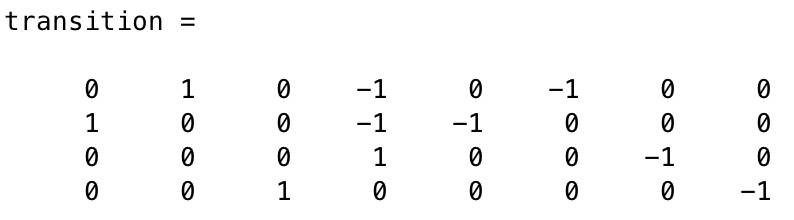
\includegraphics[width=7cm]{transition}
\caption{the transition matrix for this stochastic system.}
\label{fig:transition} 
\end{figure}

For each reaction type, the mean time till the next reaction occurs again is the inverse of the reaction rate.  Since the rate at which anything will happen is simply the sum of all the reaction rates, which we'll denote by $\lambda$, we also can write the mean time until any reaction occurs as   

\begin{figure}[ht]
\centering
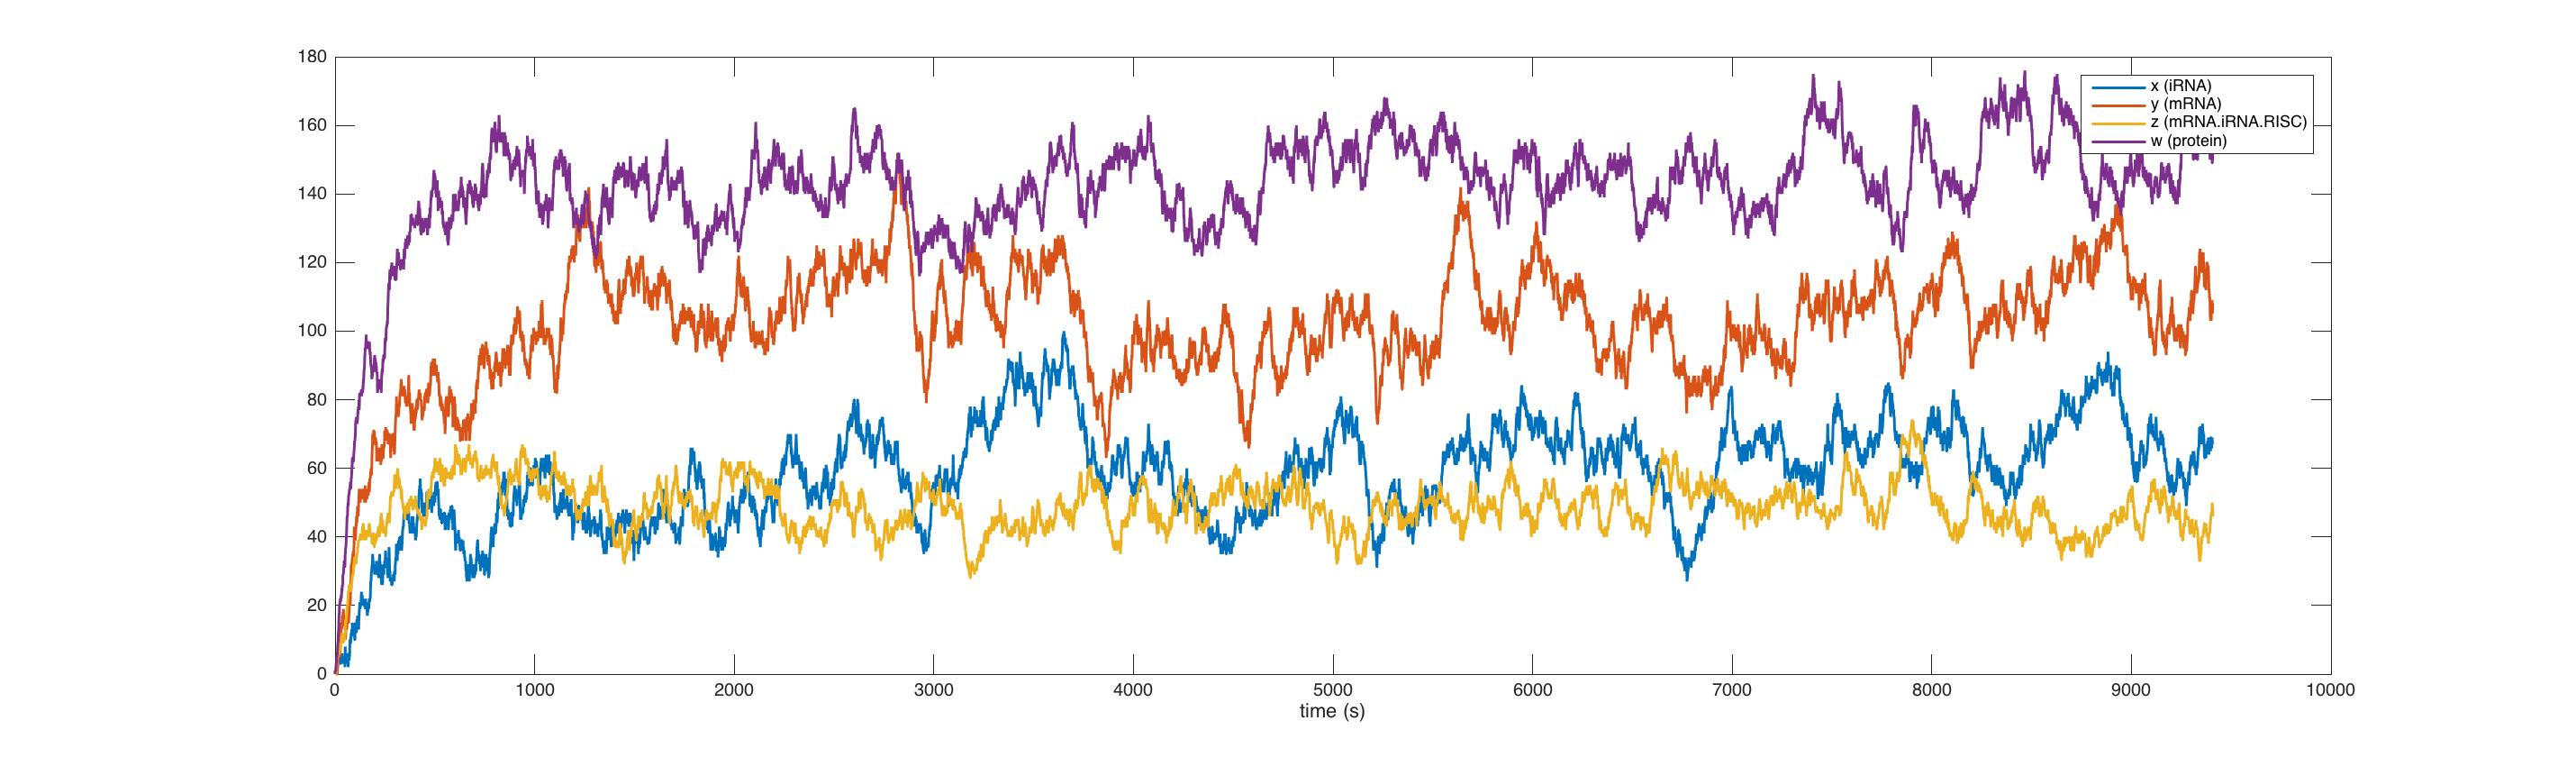
\includegraphics[width=\linewidth]{stochsim}
\caption{the stochastic dynamics of the system of mRNA, iRNA and protein along time.}
\label{fig:stochsim} 
\end{figure}

\begin{figure}[ht]
\centering
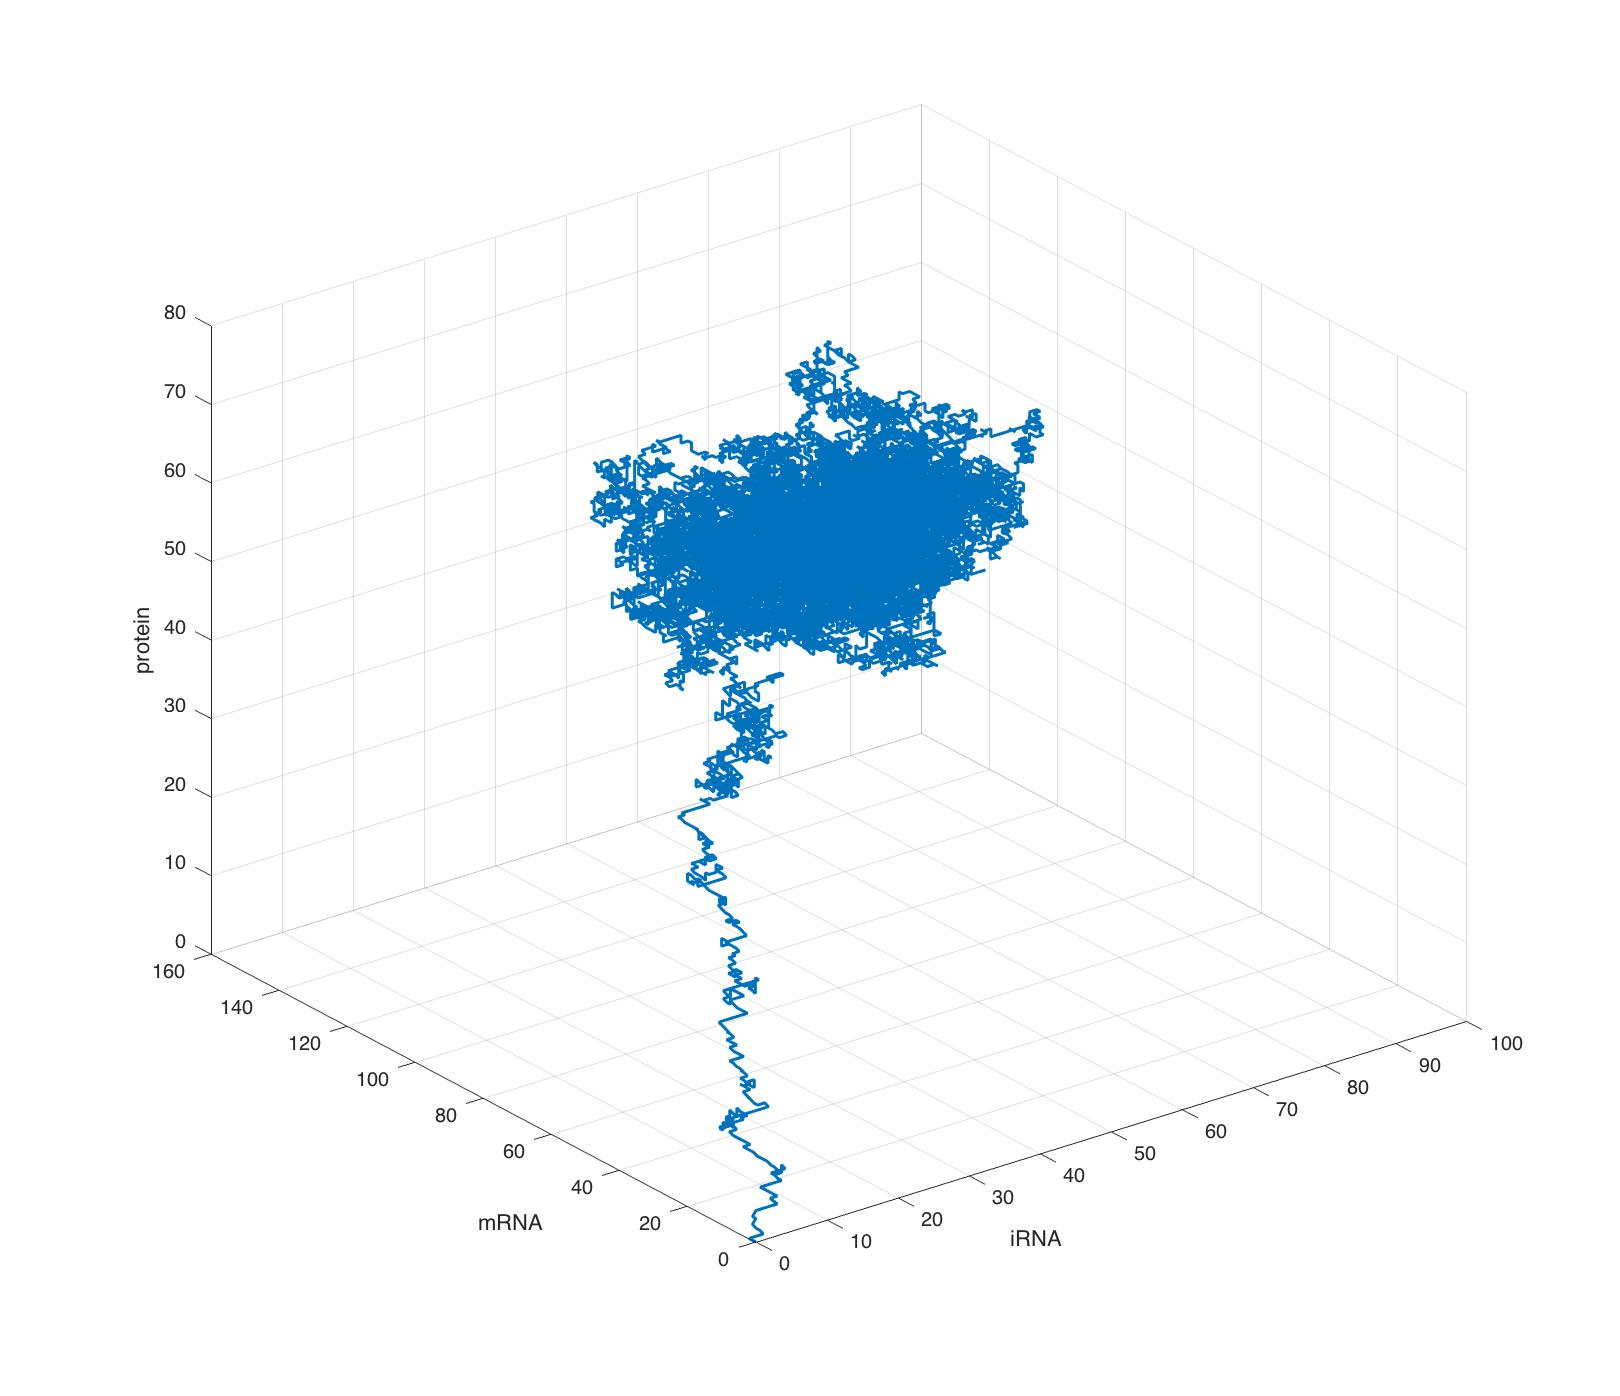
\includegraphics[width=\linewidth]{gridstochsim}
\caption{the stochastic relationship of mRNA, iRNA and protein along time.}
\label{fig:gridstochsim} 
\end{figure}

As shown in Figure \ref{fig:stochsim}, the stochastic behavior is well captured in this Monte Carlos simulation in considerable amount of run time. Similar to the specified chemical master equation, the stochastic relationship of the system is shown in Figure \ref{fig:gridstochsim} , starting from (0, 0, 0), departing towards an equilibrium region.

\section*{Discussion}

As shown from our investigation, the system tends to reach an equilibrium steady state within certain amount of time. The chemical master equation captures the single-molecule event in a precise level (Figure \ref{fig:deterdyn}). However, the lack of experimental understanding of the probability distribution of the mRNA, iRNA and protein in a single-molecule level prevent us from developing probability generating functions, which can gave us a better understanding of the whole picture. Despite this unfeasible attempt, another attempt to introduce single-molecule stochastic dynamics based on a waiting time model was well constructed under the assumption of a Poisson distribution. The Monte Carlos simulation based on this stochastic model captured this behavior and demonstrated the predicted equilibrium behavior (Figure \ref{fig:stochsim}). Figure \ref{fig:gridstochsim}) is also a nice representation of how our chemical master equation can be simulated with more probability generating information.

Based on our model, more detailed investigation can be conducted. Specific types of microRNA can have cascade-like genetic circuits as well as specific bound RNA sequences, which implies combinatorial structures of signaling. We can also consider an introduction of transcription factor, in order to observe the interactions between this two types of regulations. Another improvement would be reducing our assumptions one by one.

Further exploration can be also expanded to the stochastic modeling long noncoding RNA (LncRNA)’s “origami-like” interaction with DNA and RNA in a 3D single-molecule biophysics perspective, which can be very beneficial to future bioengineering regarding disease and development. With the same genomic code, the massive cellular diversity might be just encoded by regulation of different noncoding RNA. Some promising future attempt would be including the noncommutative sequential regulation in which a time-evolving origami can generate diversity in biological systems.

\bibliography{./sample}

\section*{Acknowledgments}

Thank Prof. Qian for giving us insightful lectures about the mathematical theories of cellular dynamic and the exciting field of mathematical biology. Thank him for always setting challenging questions for me to explore! Thank my friends in AMATH 531 who come along with me in great energy! Thank University of Washington for giving me the platform to scientifically explore problems and subjects! I will continue the voyage of exploring the infinite realm of mathematical and systems biology in my academic career fearlessly.

\section*{Additional information}

For supporting MATLAB Codes, please refer to Supplementary Information Attached. All code for the reproduction of the reported results can be downloaded from my \href{https://github.com/doerlbh/RNAi_CME_Dynamics}{GitHub Repository}.

\section*{Supplementary information}

Supporting MATLAB codes are attached below:

\begin{lstlisting}

% RNA interference modeled by Deterministic ODE
% Author: Baihan Lin
% Date: Nov 2016

clear all; close all

gm1 = 0.3;
gm2 = 0.8;
gm3 = 0.2;
K1 = 0.3;
K2 = 0.5;
H = 0.5;

ep1 = gm2/gm3;
ep2 = gm1/gm3;
H1 = H*K1/(gm1*gm3);
H2 = H*K2/(gm1*gm3);
H3 = H^2*ep1*K1*K2/(gm2^2);

%% Dynamic Simulation

for numreps=1:1

p = [ep1, ep2, H1, H2, H3];
x0 = [0, 0, 0, 0];

Tmax=5;
options = odeset('NonNegative',1:4); %make solutions nonnegative

[T,Y] = ode45(@(t,y) iRNA_ODE(t,y,p),[0 Tmax],x0,options);

figure(1)
subplot(2,1,1);
plot(T,Y(:,1:2),'LineWidth',1.5);
legend('v (iRNA)','r (mRNA)')
xlabel('t'); 
ylabel('nondimensionalized mRNA/iRNA');

subplot(2,1,2);
plot(T,Y(:,4),'LineWidth',1.5); hold on;
legend('s (protein)')
xlabel('t'); 
ylabel('nondimensionalized protein');

figure(2)
grid on;
set(gca,'FontSize',16)
plot3(Y(:,1),Y(:,2),Y(:,4),'LineWidth',1.5);
xlabel('v (iRNA)'); 
ylabel('r (mRNA)');
zlabel('s (protein)');

end

%% Steady States Search

v = 0:0.01:1;
r = 0:0.01:1;
vpre = 1+H1*r;
rpre = 1+H2*v;
vnull = 1./vpre;
rnull = 1./rpre;

v_star = (H2-H1-1+sqrt((H2-H1-1)^2+4*H2))/(2*H2);
r_star = (H1-H2-1+sqrt((H1-H2-1)^2+4*H1))/(2*H1);

figure(3)
plot(v, rnull,'LineWidth',1.5);hold on
plot(vnull,r,'LineWidth',1.5);
plot(v, r_star*ones(1,length(v)), '.r');
plot(v_star*ones(1,length(v)), r, '.r');
plot(v_star,r_star,'o');
legend('r nullcline', 'v nullcline');
xlabel('v (iRNA)'); 
ylabel('r (mRNA)');


\end{lstlisting}

\begin{lstlisting}

% RNA interference modeled by Deterministic ODE
% Author: Baihan Lin
% Date: Nov 2016

%  dvdt = ep1 * (1 - v - H1 * v * r);
%  drdt = ep1 * (1 - r - H2 * v * r);
%  dqdt = ep2 * (- q + H3 * v * r);
%  dsdt = r - s;

function dy = iRNA_ODE(t,y,p)

ep1 = p(1);
ep2 = p(2);
H1 = p(3);
H2 = p(4);
H3 = p(5);

dy = zeros(4,1);

dy(1) = ep1 * (1 - y(1) - H1 * y(1) * y(2));
dy(2) = ep1 * (1 - y(2) - H2 * y(1) * y(2));
dy(3) = ep2 * (- y(3) + H3 * y(1) * y(2));
dy(4) = y(2) - y(4);

end


\end{lstlisting}

\begin{lstlisting}

% RNA interference modeled by Monte Carlos Simulation
% Author: Baihan Lin
% Date: Nov 2016

clear all; close all

gm1 = 0.005;
gm2 = 0.01;
gm3 = 0.006;
K1 = 1;
K2 = 0.8;
K3 = 0.9;
H = 0.5;
f = 0.3;

% ep1 = gm2/gm3;
% ep2 = gm1/gm3;
% H1 = H*K1/(gm1*gm3);
% H2 = H*K2/(gm1*gm3);
% H3 = H^2*ep1*K1*K2/(gm2^2);

p = [gm1, gm2, gm3, K1, K2, K3, H, f];
x0 = [0; 0; 0; 0];

rng(1);

Nstep=50000;
stptime = zeros(Nstep,1);
time = zeros(Nstep,1);
xall = zeros(Nstep,4);
xall(1,:) = x0;
x = x0;

for step = 1 : Nstep - 1
   [xnew, tau] = stoch_update(x, p);
   x = xnew;
   stptime(step+1) = tau;
   time(step+1) = time(step) + tau;
   xall(step+1,:) = x;
end

figure(1)
plot(time,xall(:,1:4),'LineWidth',1.5);
legend('x (iRNA)','y (mRNA)','z (mRNA.iRNA.RISC)','w (protein)');
xlabel('time (s)'); 
% 
% figure(2)
% plot(1:Nstep,xall(:,1:4),'LineWidth',1.5);
% legend('x (iRNA)','y (mRNA)','z (mRNA.iRNA.RISC)','w (protein)');
% xlabel('steps'); 

figure(3)
plot3(xall(:,1),xall(:,2),xall(:,3),'LineWidth',1.5);
grid on
xlabel('iRNA'); 
ylabel('mRNA'); 
zlabel('protein'); 

\end{lstlisting}

\begin{lstlisting}

% RNA interference modeled by Stochastic Monte Carlos
% Author: Baihan Lin
% Date: Nov 2016

function [ynew, tau] = stoch_update(y, p)

gm1 = p(1);
gm2 = p(2);
gm3 = p(3);
K1 = p(4);
K2 = p(5);
K3 = p(6);
H = p(7);

rates = [K1;
    K2;
    K3;
    H;
    gm1*y(2);
    gm1*y(1);
    gm2*y(3);
    gm3*y(4)];

lambda = sum(abs(rates));

transition = [0 1 0 -1 0 -1 0 0;
    1 0 0 -1 -1 0 0 0;
    0 0 0 1 0 0 -1 0;
    0 0 1 0 0 0 0 -1];

ynew = y;

tau = log(1/rand()) / lambda;

r = rand()*lambda;

current = 0;
selection = 1;

for it = 1:length(rates)
    current = current + rates(it);
    if current > r
        selection = it;
        disp(selection);
        break;
    end
end

ynew
ynew = ynew + transition(:,selection);
ynew = ynew.*[ynew >= 0];

end

\end{lstlisting}

\end{document}